\section{Структура программ и языков в среде "<MPS">}
Каждой конструкции программы в среде "<MPS"> соответствует узел АСГ. Узел может содержать:
\begin{itemize}
 \item простые свойства, например, имя у переменной или значение у числовой константы;
 \item дочерние узлы, если в состав соответствующей конструкции входят другие конструкции, например, операнды бинарной операции;
 \item ссылки на другие узлы АСГ, например, узел, соответствующий использованию переменной, ссылается на узел, соответствующий декларации переменной.
\end{itemize}

Например, выражению "<i < 10"> соответствует фрагмент АСГ, представленный на рисунке \ref{fig:Less}.
\begin{figure}
 \centering
 \fbox{
  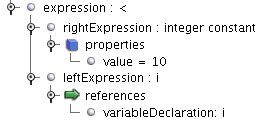
\includegraphics{Less.png}
 }
 \caption{Фрагмент АСГ, соответствующий выражению "<i < 10">}
 \label{fig:Less}
\end{figure}

Никуда не вложенные узлы называются корневыми. Корневые узлы соответствуют модулям-файлам в текстовых языках программирования. Каждый корневой узел вместе со всеми вложенными в него узлами принадлежит некоторой модели. Каждая модель, в свою очередь, принадлежит некоторому модулю. Модули бывают нескольких типов. Наиболее важными среди них являются решения (solution) и языки.

Решения представляют собой законченные программы или подсистемы программ, написанные с использованием различных языков, разработанных в среде "<MPS">.

Модели, входящие в состав языка, описывают различные аспекты этого языка: абстрактный и конкретный синтаксис, систему типов, операционную семантику и т.п. Следует отметить, что для описания всех этих аспектов также созданы проблемно-ориентированные языки, и, более того, применен принцип раскрутки, то есть эти языки переписаны уже при помощи самих себя.

Каждому типу языковых конструкций соответствует ровно одна декларация типа узла. Типы узлов в среде "<MPS"> называются "<концептами">. Новый термин введен для того, чтобы отличать понятие для типа узла от понятий "<типа"> и "<класса">, которые имеют свой собственный смысл во многих языках программирования. Концепт узла, соответствующего некоторой конструкции, также является узлом и находится в специальной модели того языка, которому принадлежит эта конструкция. Например, концептом конструкции "<i < 10"> является корневой узел "<LessThanExpression">, находящийся в модели "<structure"> языка "<jetbrains.mps.baseLanguage"> \pic{\ref{fig:LessThenExpressionConcept}}.

\begin{figure}
 \centering
 \fbox{
  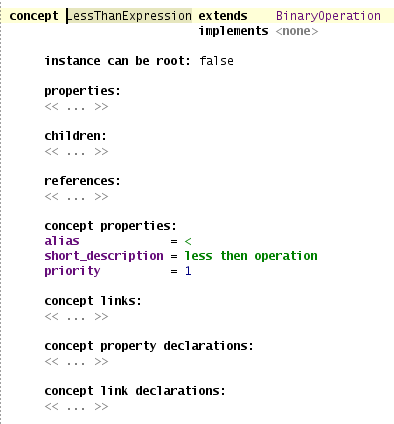
\includegraphics{LessThanExpressionConcept.png}
 }
 \caption{Концепт конструкции "<меньше">}
 \label{fig:LessThenExpressionConcept}
\end{figure}


Таким образом, на мета-уровне у узла может быть два типа ссылок: узел может ссылаться на другие узлы, как, например, "<использование переменной">, ссылается на "<декларацию переменной">; и узел является экземпляром некоторого концепта, как узел, соответствующий конструкции "<i < 10">, является экземпляром концепта "<LessThanExpression">.

У каждой модели есть явно заданный набор используемых языков и набор импортированных моделей. Модель может содержать только те узлы, которые являются экземплярами концептов набора используемых ею языков.

Узлы могут ссылаться друг на друга внутри одной модели. Кроме того, узел из одной модели может ссылаться на узел из другой модели. Для этого вторая модель должна быть импортирована в первую.

Концепт в среде "<MPS"> может иметь мета-свойства и мета-отношения, составляющие его мета-структуру. Мета-структура используется при описании аспектов языка, но не при программировании на нем.
